\section{Constructive Heuristics}
\label{sec:heuristics}

One of the first important steps in a genetic algorithm is to construct an initial population (see Section 2.2). This can be done by generating solutions randomly or by using heuristics. The latter approach causes additional computational costs, but it guarantees that the first generation has at least several reasonably good solutions. \par
 
This chapter gives an overview of heuristics \cite{knust2020script} which will be used in our research as a basis to construct an initial population for genetic algorithms. We have chosen four heuristics which are all of the constructive type because construction heuristics find feasible solutions in relatively short time. Please note that the generated solutions are not guaranteed to be optimal -- if they were, we would not need to apply a genetic algorithm.\par 

Constructive heuristics build the tour successively and greedily by using deterministic construction rules without trying to improve the existing partial tour.  We will use the term "partial tour" in the following to denote the part of the resulting tour which has already been built. Please note that it is important for these heuristics which city will be visited first because the solutions differ dependent on which starting point is chosen. Moreover, please note that the tour is given in the path representation here.\par

We will use the following four heuristics: nearest neighbor, double nearest neighbor, nearest insertion, and farthest insertion. They are described in detail below.

\subsection{Nearest Neighbor}
\label{subsec:nn}

Considering a partial tour is already built, the nearest neighbor (NN) heuristic iteratively chooses a city which is closest to the last city of the tour and inserts it at the end.

The algorithm includes the following steps:
\begin{enumerate}
	\item Choose an arbitrary city $\pi_{1}$ as a starting point for the current partial tour $\pi:= (\pi_{1})$.
	\item  While there are unvisited cities left:
	\subitem Given the partial tour $\pi:= (\pi_{1}, ..., \pi_{t})$, find the next unvisited city $\pi_{k} \notin \pi$ which is nearest to the city $\pi_{t}$ and add it to the partial tour such that $\pi:= (\pi_{1}, ..., \pi_{t}, \pi_{k})$.
	
\end{enumerate}

For instance, consider the five cities with symmetric distances from Table \ref{7_1_distance_table}. Let us use city A as the start city, resulting in an initial partial tour $\pi = (A)$. The next unvisited city which has the smallest distance to city A is city C with a distance of 4. We add this city after city A getting a partial tour $\pi = (A, C)$. The nearest unvisited neighbor of city C is city D  with the distance 5. Now the tour consists of three cities: $\pi = (A, C, D)$. The next unvisited city which is closest to city D is city E with a distance of 4. The partial tour is now $\pi = (A, C, D, E)$. City B is the last unused city having a distance of 10 to city E resulting in a tour $\pi = (A, C, D, E, B)$ (see Figure \ref{7_1_NN_start_1}) with the total costs $c(\pi) = 32$ including the distance between city B and A (i.e., 8). If we start with city C,  the NN heuristic results in the round tour $\pi' = (C, A, B, D, E)$ (see Figure \ref{7_2_DNN_start_2}) with the total costs $c(\pi') = 4 + 8 + 7 + 4 + 6 = 29$ which is shorter than the previous one. This illustrates the sensitivity of the construction heuristics to the start city.

\begin{table}[htp] \centering
	\centering
	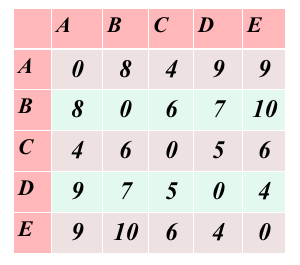
\includegraphics[width=0.3\textwidth]{7_1_distance_table}
	\caption{Distance table for five cities.}
	\label{7_1_distance_table}
\end{table}


\begin{figure}[htp] \centering
	\centering
	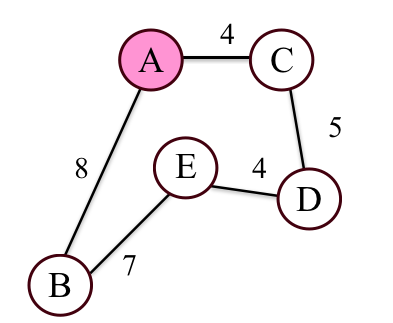
\includegraphics[width=0.3\textwidth]{7_1_NN_start_1}
	\caption{Nearest neighbor resulting tour for an example with five cities with distances in Table \ref{7_1_distance_table} and start city A.}
	\label{7_1_NN_start_1}
\end{figure}


\subsection{Double Nearest Neighbor}
\label{subsec:dnn}
The double nearest neighbor (DNN) heuristic is a modified version of the NN heuristic: It looks for a neighbor which is closest to either the first or the last city of the existing partial tour. This neighbor will be inserted before the first city or after the last city, respectively. The DNN algorithm includes the following steps:

\begin{enumerate}
	\item Choose an arbitrary city $\pi_{1}$ as a starting point for the current partial tour $\pi:= (\pi_{1})$.
	\item  While there are unvisited cities left:
	\subitem a. Given the partial tour $\pi:= (\pi_{1}, ..., \pi_{t})$, find an unvisited city $\pi_{i} \notin \pi$ which is nearest to the first city $\pi_{1} $ and an unvisited city $\pi_{j} \notin \pi$ which is nearest to city $\pi_{t}$. Let $d(\pi_{i}, \pi_{1})$ be the distance between $\pi_{i} $ and $\pi_{1} $ and  $d(\pi_{t}, \pi_{j})$ be the distance between $\pi_{t}$ and $\pi_{j}$.
	\subitem b. If $d(\pi_{i}, \pi_{1}) < d(\pi_{t}, \pi_{j})$: Insert city $\pi_{i}$ at the beginning of the partial tour such that $\pi:= (\pi_{i}, \pi_{1}, ..., \pi_{t})$.
	\subitem c. Otherwise, if $d(\pi_{i}, \pi_{1}) \ge d(\pi_{t}, \pi_{j})$: Insert city $\pi_{j}$ at the end of 	the partial tour such that $\pi:= (\pi_{1}, ..., \pi_{t}, \pi_{j})$. 
\end{enumerate}

Let us reuse the example with the five cities from Table \ref{7_1_distance_table}. If we start with city A here, the DNN will result in the same round tour as the NN does. Therefore, we start with city C. Its nearest neighbor is city A with the distance 4, resulting in a partial tour $\pi = (C, A)$ Now we have to find unvisited cities which are nearest to cities A and C, respectively. City B is the nearest to city A with the distance 8, and city D is nearest to city C with a distance of 5. Therefore, we add city D at the beginning before city C which results in the partial tour $\pi =(D, C, A)$. The next unvisited city nearest to city D is city E with a distance of 4, while the nearest unvisited neighbor of city A is still city B. This means that city E will be added to the tour before city D resulting in $\pi =(E, D, C, A)$. The last city B will be added to the tour resulting in the round tour $\pi =(E, D, C, A, B)$. If we want the start city to be at the beginning of the tour, this can be written as $\pi =(C, A, B, E, D)$. The total costs are $c(\pi) = 4 + 8 + 10 + 4 + 5 = 31$. Figure \ref{7_2_DNN_start_2} compares the tours found by the NN and the DNN heuristics, respectively, with city C used as starting point. As we can see, the DNN is not necessarily always better than the NN, although more computations have been made.


\begin{figure}[htp] \centering
	\centering
	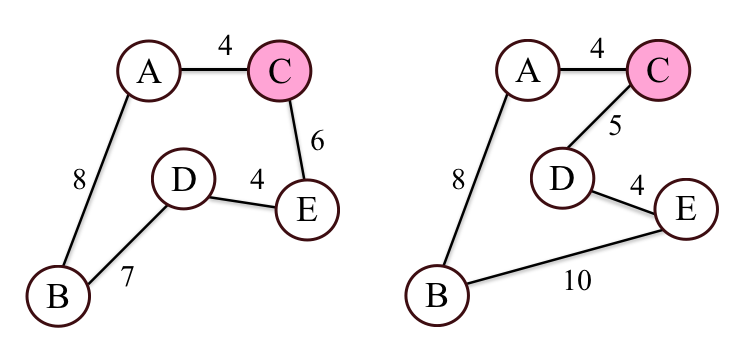
\includegraphics[width=0.5\textwidth]{7_2_DNN_start_2}
	\caption{Tours found by the NN heuristic (left) with costs 29 and the DNN heuristic (right) with costs 31, both starting with city C for an example with five cities with distances from Table \ref{7_1_distance_table}.}
	\label{7_2_DNN_start_2}
\end{figure}


\subsection{Nearest Insertion}
\label{subsec:ni}

Generally speaking, the nearest insertion algorithm (NI) looks iteratively for an unvisited city which is closest to \textit{any} city from the partial tour and inserts this city in the tour at the position where the insertion costs are minimal. If considered in detail, the steps are the following:

\begin{enumerate}
	\item Choose an arbitrary city $\pi_{1}$ as a starting point for the partial tour $\pi:= (\pi_{1})$.
	\item While there are unvisited cities left: 
	\subitem a. Let us assume that the partial tour is given as $\pi:= (\pi_{1}, ..., \pi_{t})$. For each unvisited city $\pi_{j} \notin \pi$ calculate the distance $d_{\pi}(\pi_{j})$ to the partial tour $\pi$ which is defined as $d_{\pi}(\pi_{j}) := \min _{i = 1}^{t}d({\pi_{j}, \pi_{i}})$.
	\subitem b. Choose city $\pi_{j}^{*} \notin \pi$ with the smallest distance $d_{\pi}(\pi_{j}^{*} )$.
	\subitem c. Insert city $\pi_{j}^{*}$ between those neighbor cities $\pi_{l} \in \pi$ and $\pi_{l + 1} \in \pi$, where the insertion costs $c(\pi_{l}, \pi_{j}^{*}, \pi_{l + 1}) := d(\pi_{l}, \pi_{j}^{*}) + d(\pi_{j}^{*}, \pi_{l + 1}) - d(\pi_{l}, \pi_{l + 1})$ are the smallest.
\end{enumerate}

\begin{figure}[htp] \centering
	\centering
	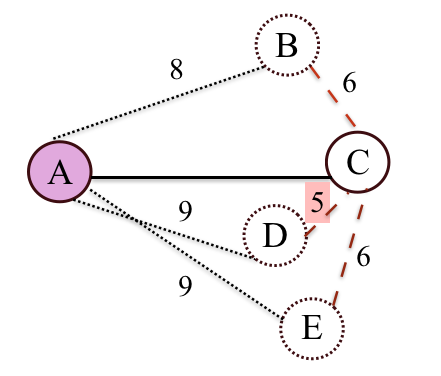
\includegraphics[width=0.4\textwidth]{7_3_part_tour_AC}
	\caption{Distances to the partial tour $\pi = (A, C)$ for cities B, D, and E (on red dashed lines).}
	\label{7_3_part_tour_AC}
\end{figure}

\begin{figure}[htp] \centering
	\centering
	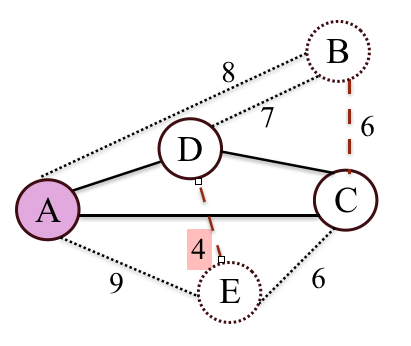
\includegraphics[width=0.4\textwidth]{7_3_part_tour_ADC}
	\caption{Distances to the partial tour $\pi = (A, D, C)$ for cities B and E (on red dashed lines).}
	\label{7_3_part_tour_ADC}
\end{figure}

Let us again consider the example with five cities with distances given in Table \ref{7_1_distance_table}. We will start with city A giving us the initial partial tour $\pi =  ( A )$. As $\pi$ consists only of one city, we look for an unvisited city nearest to city A which is city C. We add it to the partial tour $\pi$ just after city A without calculating insertion costs, as there is only one option to insert at the moment. This results in the partial tour $\pi = (A, C)$. Now, for each unvisited city, we calculate its distance to the partial tour $\pi$: $d_{\pi}(B) = 6$, $d_{\pi}(D) = 5$, and $d_{\pi}(E) = 6$. City D has the smallest distance and will be chosen (see Figure \ref{7_3_part_tour_AC}). As there is only one pair of cities in the partial tour $\pi$, there is only one possible location for city D. This results in the partial tour $\pi = (A, D, C)$. The next unvisited city which has the smallest distance to the partial tour $\pi$ is city E (see Figure \ref{7_3_part_tour_ADC}). As there are 3 cities in the current partial tour $\pi$, there are three pairs between which city E could be inserted. The costs of inserting city E between cities A and D are $c(A, E, D) = 9 + 4 - 9 = 4$. Moreover, $c(D, E, C) = 4 + 6 - 5 = 5$ and $c(C, E, A) = 6 + 9 - 4 = 11$. Therefore, city E is inserted between cities A and D, resulting in $\pi = (A, E, D, C)$. City B is the last unvisited city. Its insertion costs are $c(A, B, E) = 8 + 10 - 9 = 9$, $c(E, B, D) = 10 + 7 - 4 = 13$, $c(D, B, C) = 7 + 6 - 5 = 8$, and $c(C, B, A) = 6 + 8 - 4 = 10$. Therefore, city B will be inserted between cities D and C, resulting in the tour $\pi = (A, E, D, B, C)$ with the total costs $c(\pi) = 9 + 4 + 7 + 6 + 4 = 30$. If the NN and DNN heuristics are started with city A as well, they both produce tours with costs 32. This illustrates that the NI heuristic can be useful.


\subsection{Farthest Insertion}
\label{subsec:fi}

The farthest insertion (FI) heuristic is almost identical to the NI heuristic. It only differs from the NI by choosing a city among the list of unvisited cities whose minimal distance to the partial tour $\pi$ is \textit{maximal}. We can thus modify the NI algorithm by replacing line $b$ with the following line $b'$:

b'. Choose city $\pi_{j}^{*}\notin \pi$ with the largest distance $d_{\pi}(\pi_{j}^{*})$.

\begin{figure}[htp] \centering
	\centering
	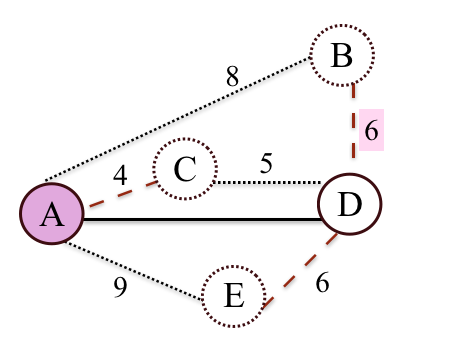
\includegraphics[width=0.4\textwidth]{7_4_part_tour_AD}
	\caption{Distances to the partial tour $\pi = (A, D)$ for cities B, C, and E (on red dashed lines).}
	\label{7_4_part_tour_AD}
\end{figure}

\begin{figure}[htp] \centering
	\centering
	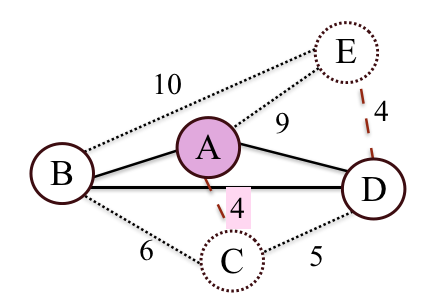
\includegraphics[width=0.4\textwidth]{7_4_part_tour_ABD}
	\caption{Distances to the partial tour $\pi = (A, B, D)$ for cities C and E (on red dashed lines).}
	\label{7_4_part_tour_ABD}
\end{figure}

While this modification may sound counter-intuitive, the following example illustrates that the FI heuristic can sometimes give better results than the NI one: Let us consider the same example with five cities and distances given in Table \ref{7_1_distance_table} with the start city A. Our initial partial tour is $\pi = (A)$. Cities D and E have the maximal distance $d_{\pi}(D)$ = $d_{\pi}(E)$ = 9 to the partial tour $\pi$. For cities with identical distance, we use the one appearing first in the alphabetical order, i.e. city D. This results immediately in the partial tour $\pi = (A, D)$, as there is only one option to insert city D. The next unvisited city with the largest distance $d_{\pi}$ to the already build partial tour $\pi$ is city B with a distance of 6 (see Figure \ref{7_4_part_tour_AD}). There is only one pair in $\pi$ now; therefore, there exists only one option to insert city B. This results in the partial tour $\pi = (A, B, D)$. Both remaining cities C and E have an identical distance $d_{\pi}(C)$ = $d_{\pi}(E)$ = 4 to this partial tour (see Figure \ref{7_4_part_tour_ABD}). We choose city C based on the alphabetical order. The insertion costs for city C are $c(A, C, B) = 4 + 6 - 8 = 2$, $c(B, C, D)  = 6 + 5 - 7 = 4$, and $c(D, C, A) = 5 + 4 - 9 = 0$. Therefore, city C will be inserted between cities D and A, resulting in $\pi = (A, B, D, C)$. The last unvisited city is city E. Its insertion costs are $c(A, E, B) = 9 + 10 - 8 = 11$, $c(B, E, D) = 10 + 4 - 7 = 7$, $c(D, E, C)= 4 + 6 - 5 = 5$, and $c(C, E, A)  = 6 + 9 - 4 = 11$. Therefore, city E will be inserted between cities D and C, resulting in $\pi = (A, B, D, E, C)$ with total costs $c_{\pi} = 8 + 7 + 4 + 6 = 4 = 29$. This tour produced by the FI is thus shorter than the one produced by the NI which had a total distance of 30.\par 

